\documentclass[twocolumn,a4j]{jsarticle}
\setlength{\topmargin}{-20.4cm}
\setlength{\oddsidemargin}{-10.4mm}
\setlength{\evensidemargin}{-10.4mm}
\setlength{\textwidth}{18cm}
\setlength{\textheight}{26cm}
\renewcommand{\figurename}{fig.}
\renewcommand{\tablename}{table }

\usepackage[top=15truemm,bottom=25truemm,left=20truemm,right=20truemm]{geometry}
\usepackage[latin1]{inputenc}
\usepackage{amsmath}
\usepackage{amsfonts}
\usepackage{amssymb}
\usepackage[dvipdfmx]{graphicx}
\usepackage{listings}
\usepackage{listings,jvlisting}
\usepackage{geometry}

\lstset{
basicstyle={\ttfamily},
identifierstyle={\small},
commentstyle={\smallitshape},
keywordstyle={\small\bfseries},
ndkeywordstyle={\small},
stringstyle={\small\ttfamily},
frame={tb},
breaklines=true,
columns=[l]{fullflexible},
xrightmargin=0zw,
xleftmargin=3zw,
numberstyle={\scriptsize},
stepnumber=1,
numbersep=1zw,
lineskip=-0.5ex
}

\makeatletter
\def\@maketitle
{
\begin{center}
{\LARGE \@title \par}
\end{center}
\begin{flushright}
{\large 報告書NO.02\quad\@date\quad\@author}
\end{flushright}
\par\vskip 1.5em
}
\makeatother

\author{来代 勝胤}
\title{令和3年度 5月 報告書}
\date{2021/6/2}

\begin{document}
\maketitle
\section*{\large 報告内容}
\begin{itemize}
    \item 進捗概要
    \item OpenFOAMでの解析練習
    \item 今後の予定
\end{itemize}
\section{\large 進捗概要}
5月は実験環境における流れ場の数値解析を目標にOpenFOAMを用いて解析練習を行った.
\section{\large OpenFOAMでの解析練習}
数値計算を行うことのできたモデル及び条件は以下の3例である.
なお,今回の解析条件はチュートリアル内の"motorbike"を参考に設定した.
\renewcommand{\labelenumi}{(\alph{enumi})}
\begin{enumerate}
    \item タイヤモデル単体の解析(回転なし)
    \item タイヤモデル単体の解析(回転あり)
    \item ホイールハウスを含むモデルの解析
\end{enumerate}
\subsection{OpenFOAMにおける解析の流れ}
OpenFOAMを使用した解析は以下のような流れで行った.
\begin{figure}[htbp]
    \begin{center}
        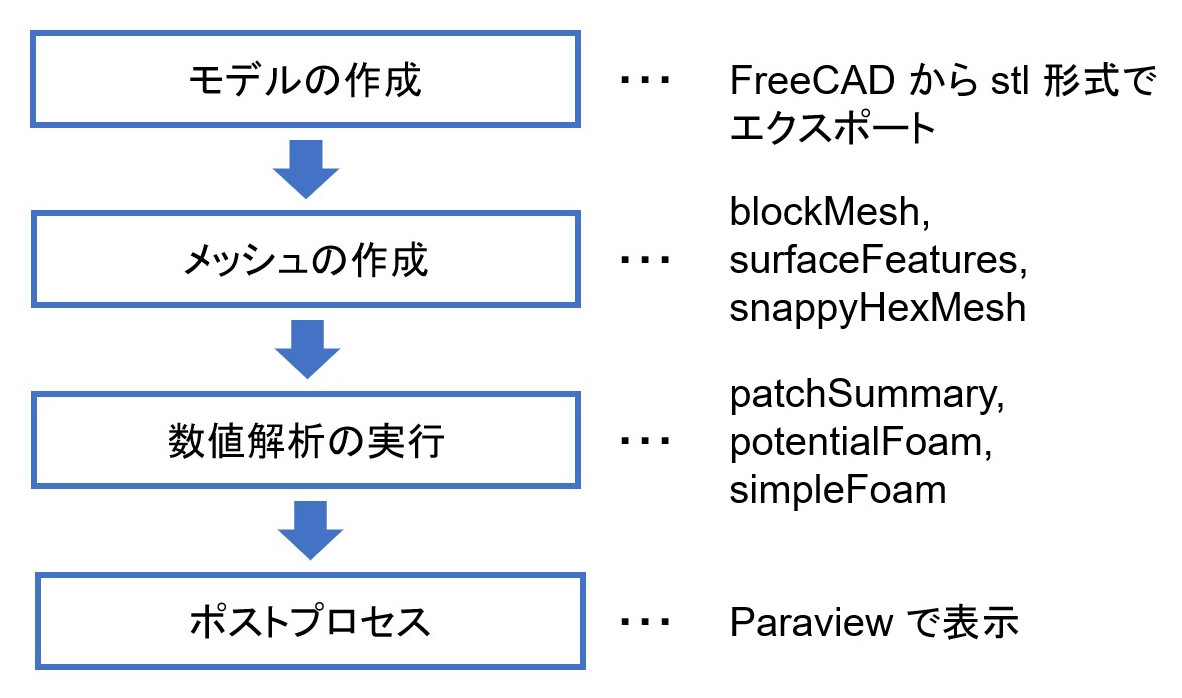
\includegraphics[width=70mm]{images/image_1.jpg}
        \caption{analysis process}
    \end{center}
\end{figure}
\subsection{解析条件}
境界条件は右上のtable 1$\sim$table 3のように設定し,計算回数は500回とした.
また,レイノルズ数は,摂氏20度における水の動粘度係数を採用し,
$\nu = 1.004 × 10^{-6} \left[\mathrm{m^2/s}\right]$
とした.
\begin{table}[htbp]
    \begin{center}
        \caption{analysis condition of stopped tyre model}
        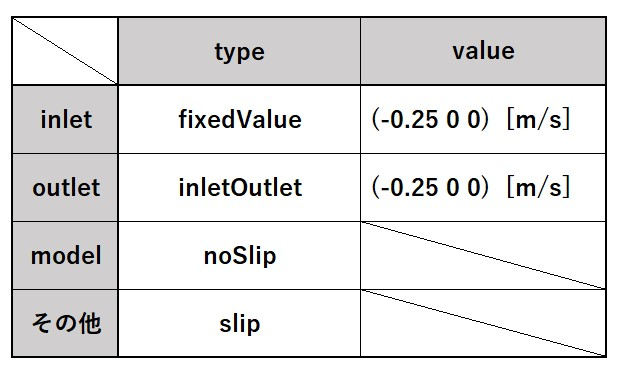
\includegraphics[width=50mm]{images/image_2.jpg}
    \end{center}
\end{table}
\begin{table}[htbp]
    \begin{center}
        \caption{analysis condition of rotating tyre model}
        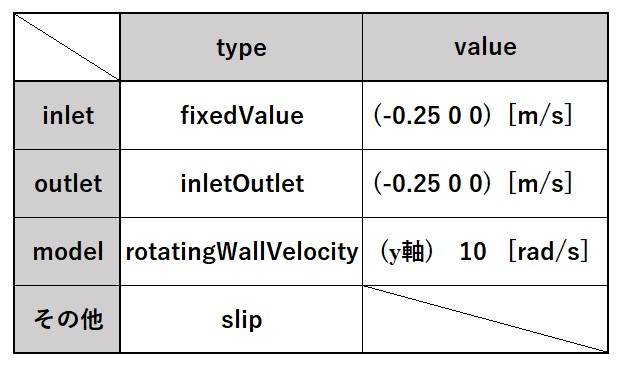
\includegraphics[width=50mm]{images/image_3.jpg}
        \caption{analysis condition of full model}
        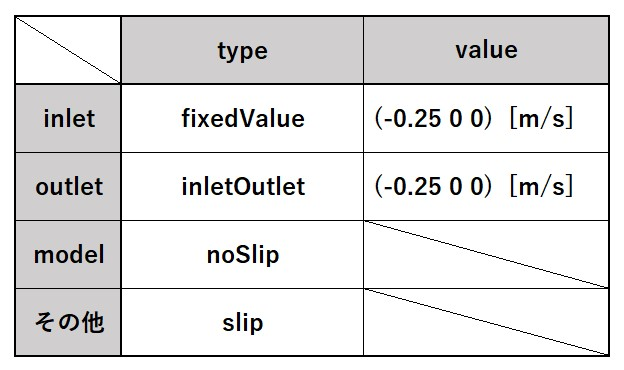
\includegraphics[width=50mm]{images/image_4.jpg}
    \end{center}
\end{table}

\newpage
\subsection{メッシュの生成}
解析領域は,$(x, y, z) = (2000, 600, 600) \left[ \mathrm{mm} \right]$を設定し,$(500, 300, 0)$の位置にモデルを設置している.
最大要素数は200,000要素とした.
\begin{figure}[htbp]
    \begin{center}
        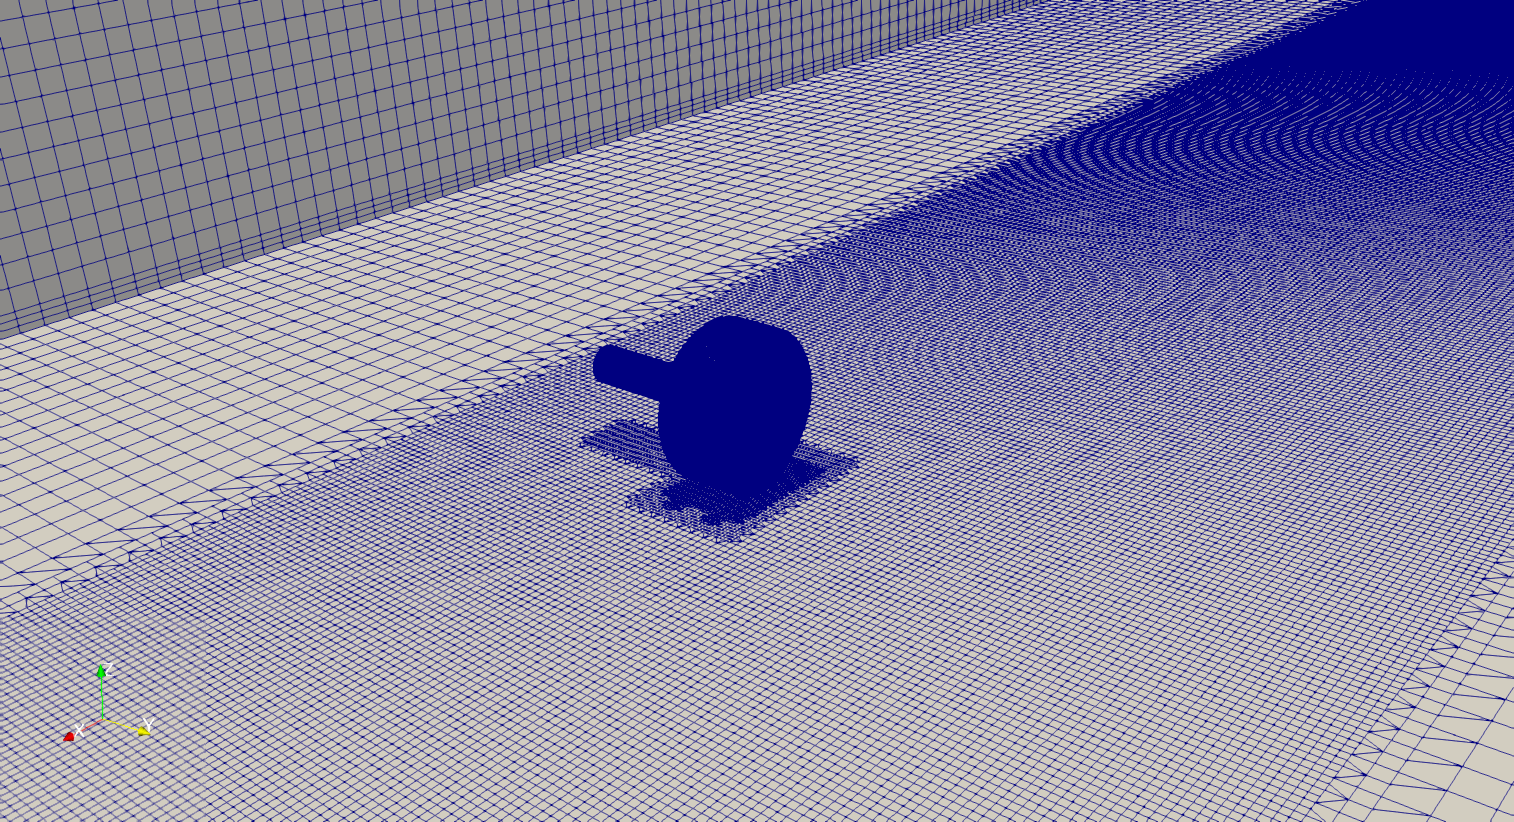
\includegraphics[width=70mm]{screenshots/tyremodel_mesh.png}
        \caption{tyre model mesh}
        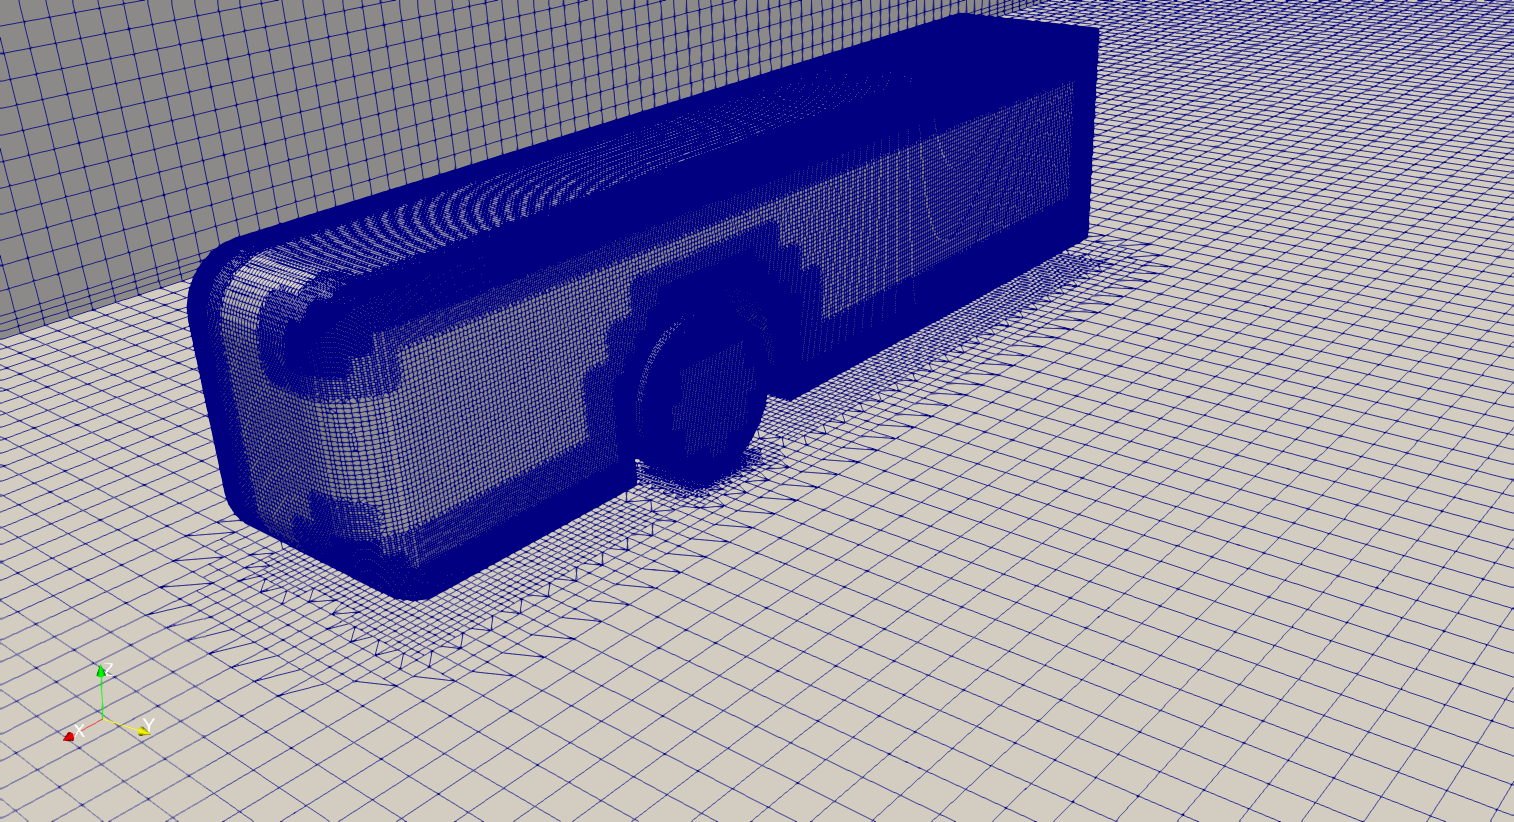
\includegraphics[width=70mm]{screenshots/fullmodel_mesh.png}
        \caption{full model mesh}
    \end{center}
\end{figure}
モデルの原点のズレがあるが,上記の2枚は同じ画角から画像を取得している.
fig.2については,モデル周りの流れを可能な限り再現するために,
タイヤモデルの前方50mmから後方150mmまでのメッシュ部分を細分化した.
同様に,fig.3のモデルにも細分化領域を指定したsnappyHexMeshDictを使用したが,
メッシュの細分化が行われなかった.なお,細分化領域についてはモデル(c)が十分に収まる領域を指定している.
\par
複数回同様の条件でメッシュの作成を行ったが,改善されることはなかった.
最大要素数の影響も考えられるため,今後条件を変更して実行する予定である.

\newpage
\subsection{解析結果}
\subsubsection{モデル(a)とモデル(b)の比較}
モデル(a)とモデル(b)について,タイヤの回転条件がどのように解析結果に現れるかを確認した.
\begin{figure}[htbp]
    \begin{center}
        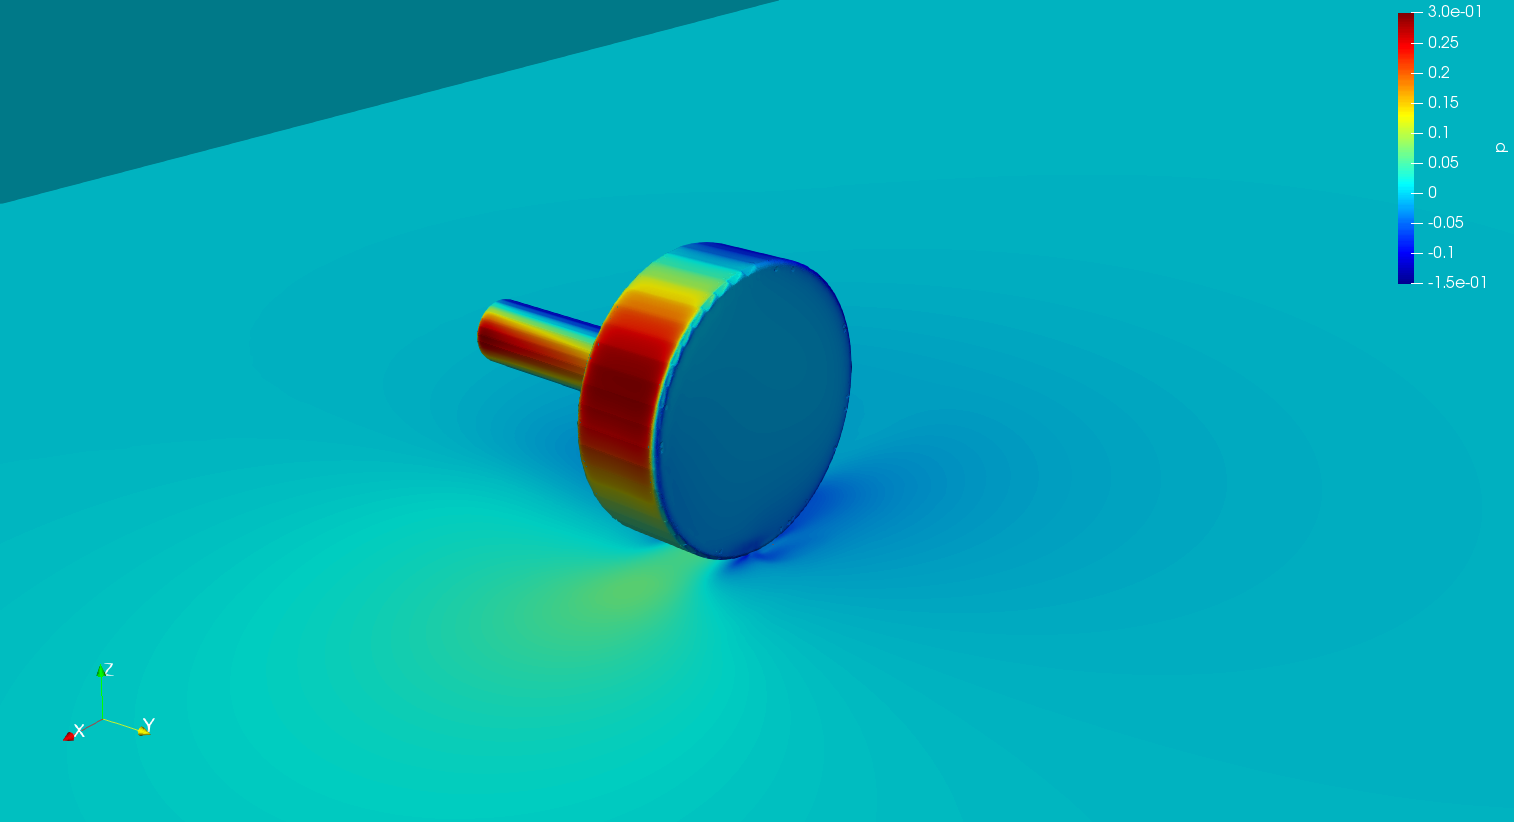
\includegraphics[width=70mm]{screenshots/tyremodel_pressure1.png}
        \caption{pressure of stopped tyre model}
        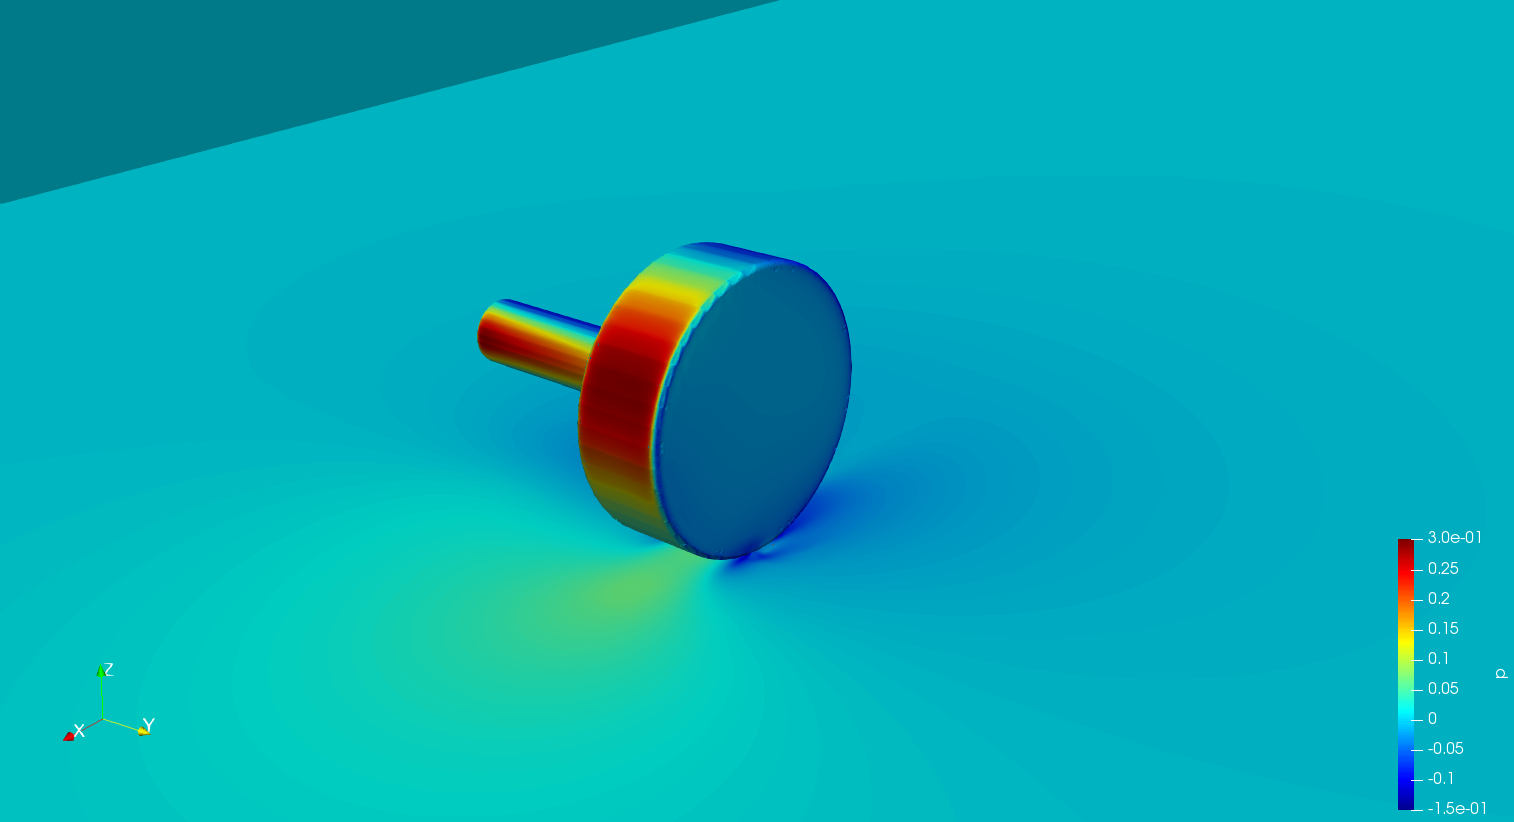
\includegraphics[width=70mm]{screenshots/tyremodel_pressure1_r.png}
        \caption{pressure of rotating tyre model}
    \end{center}
\end{figure}
\par
以上のfig.4およびfig.5をみると大きな違いは確認できなかった.
そこで,モデル表面の速度分布を表示した画像を示す.
\begin{figure}[htbp]
    \begin{center}
        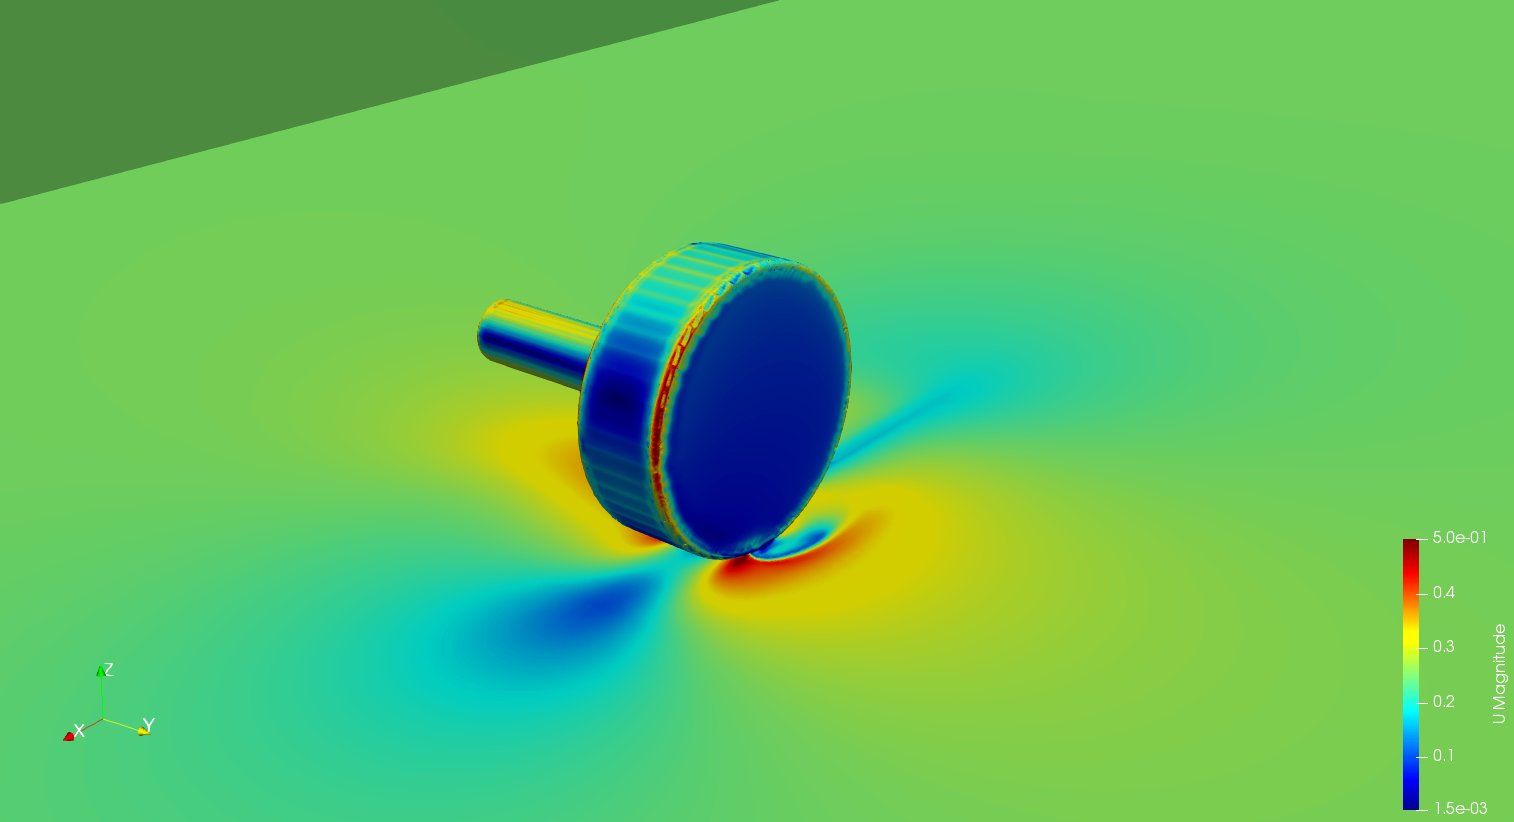
\includegraphics[width=70mm]{screenshots/tyremodel_velocity1.png}
        \caption{velocity of stopped tyre model}
        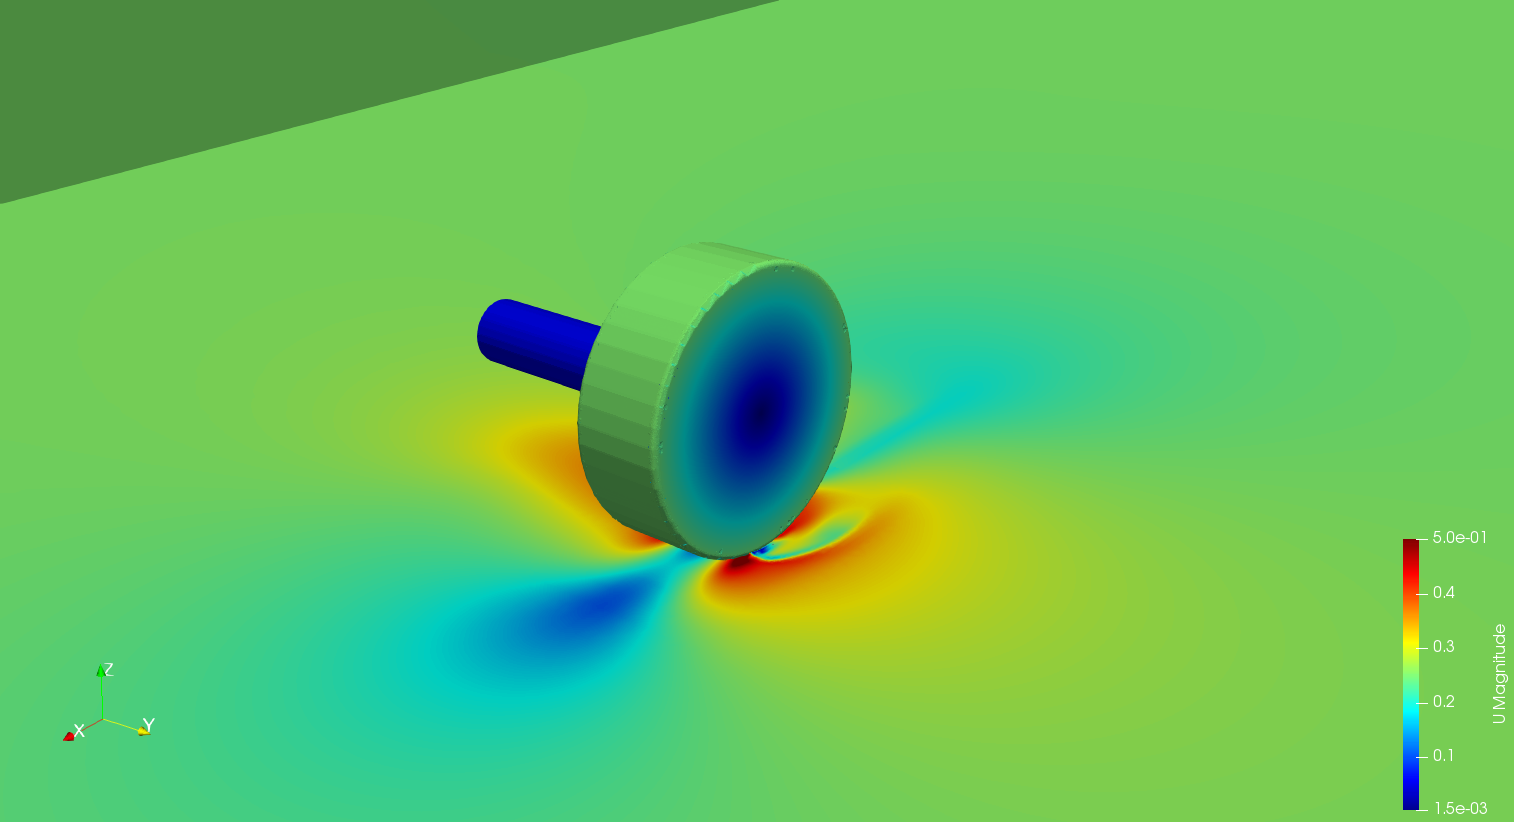
\includegraphics[width=70mm]{screenshots/tyremodel_velocity1_r.png}
        \caption{velocity of rotating tyre model}
    \end{center}
\end{figure}
\newpage
速度分布を見ると,fig.6においてモデル表面の速度分布はゼロに近くなっていることがわかる.
また,fig.7においてモデルの回転軸を中心に円形状に速度分布がみられる.
したがって,タイヤ表面における回転条件は付与されていることがわかる.
しかし,fig.6においてモデル表面に速度がゼロでない部分がみられる理由がわからなかった.
\par
次に後流の流れを流線を用いて可視化してみた・
\begin{figure}[htbp]
    \begin{center}
        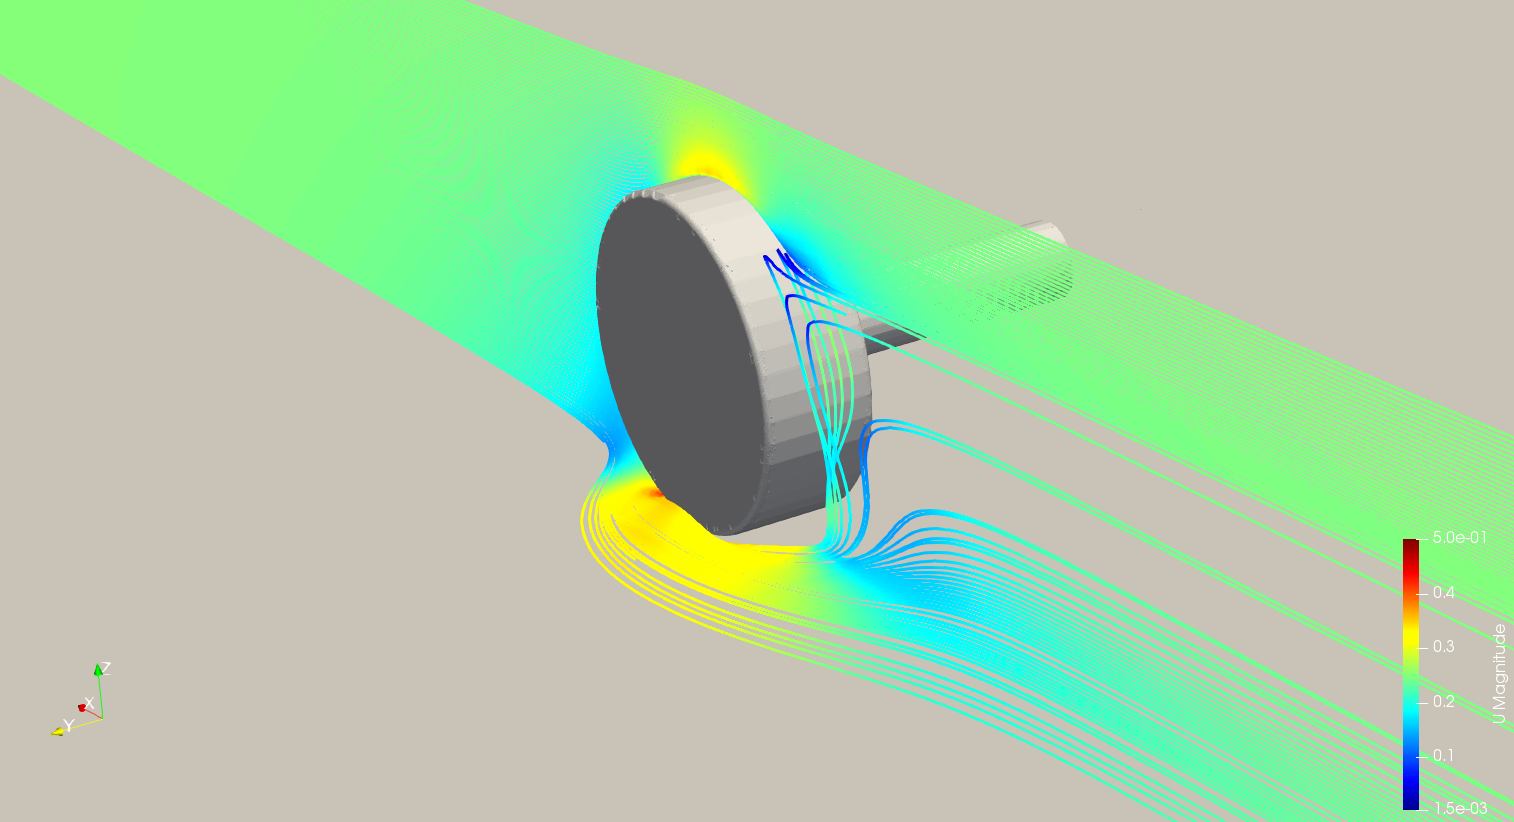
\includegraphics[width=70mm]{screenshots/tyremodel_stream2.png}
        \caption{stream of stopped tyre model}
        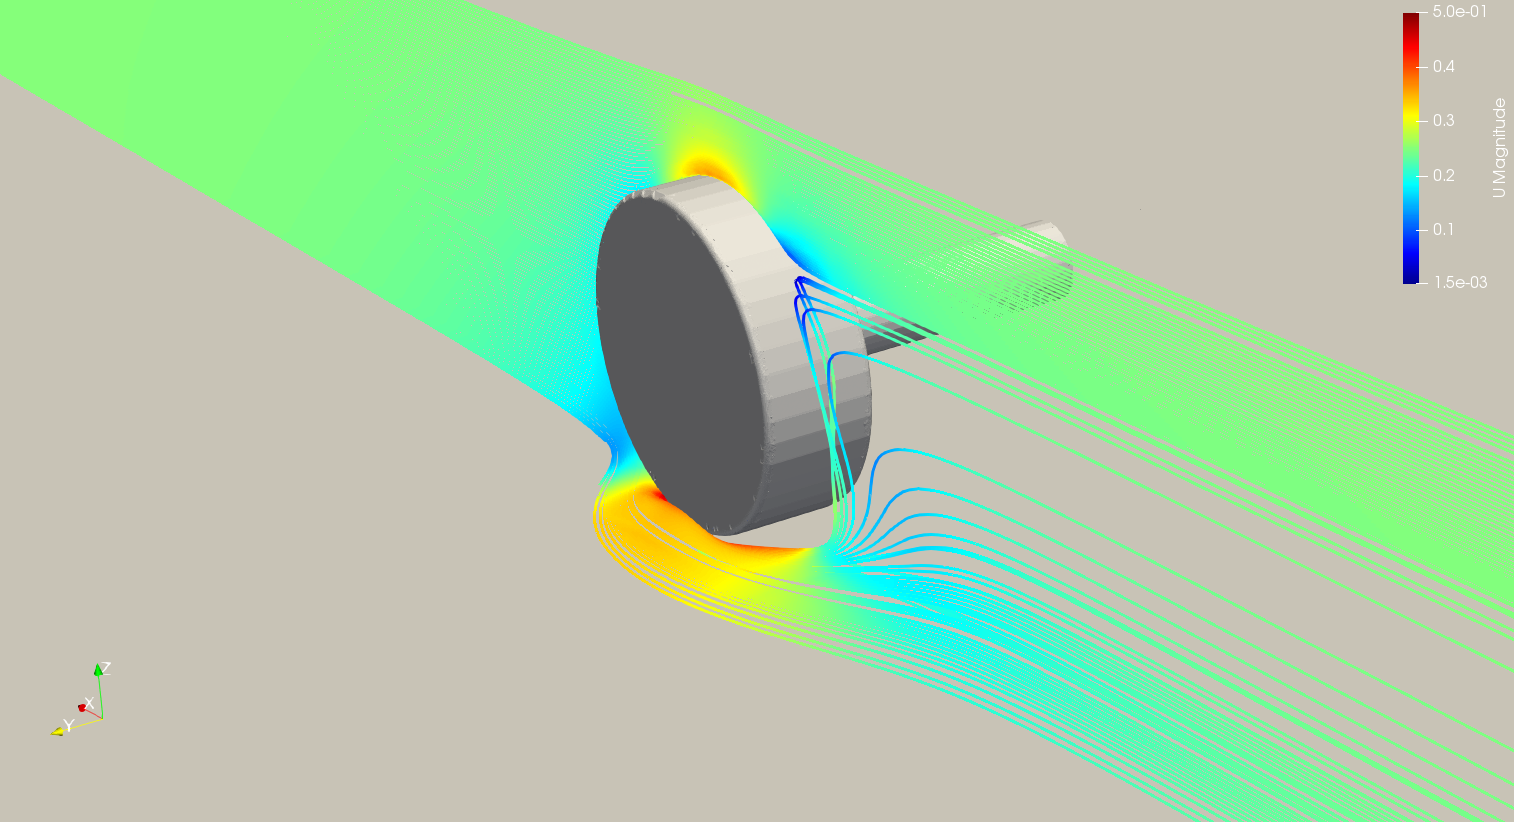
\includegraphics[width=70mm]{screenshots/tyremodel_stream2_r.png}
        \caption{stream of rotating tyre model}
    \end{center}
\end{figure}

\newpage
fig.8およびfig.9にあるように明らかな差異を確認することはできず,
モデル上部の流れ及びモデル下部の横に回り込む流れの流線の色を比較すると,
モデル(b)が微妙にモデル(a)より流速が大きいといった違いがみられる程度であった.\\
\subsubsection{モデル(c)の解析画像}
fig.3に示した細分化領域の作成されていないメッシュを使用して,
試験的に解析を行った画像を以下に示す.
今後はメッシュの細分化,タイヤモデルへの回転条件の付与を目標に解析方法を探っていきたい.
\begin{figure}[htbp]
    \begin{center}
        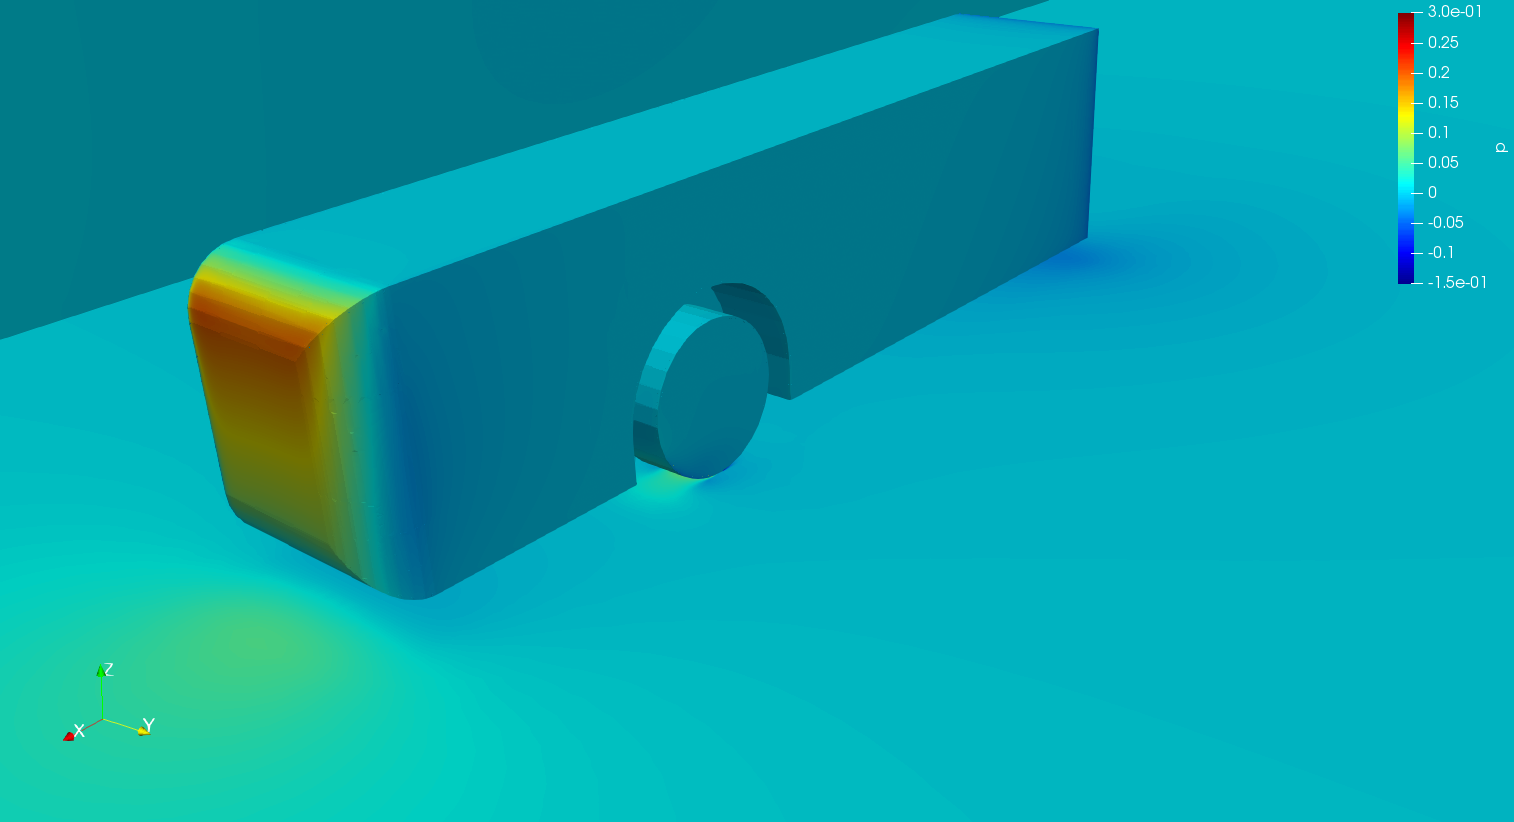
\includegraphics[width=70mm]{screenshots/fullmodel_pressure.png}
        \caption{pressure of full model}
        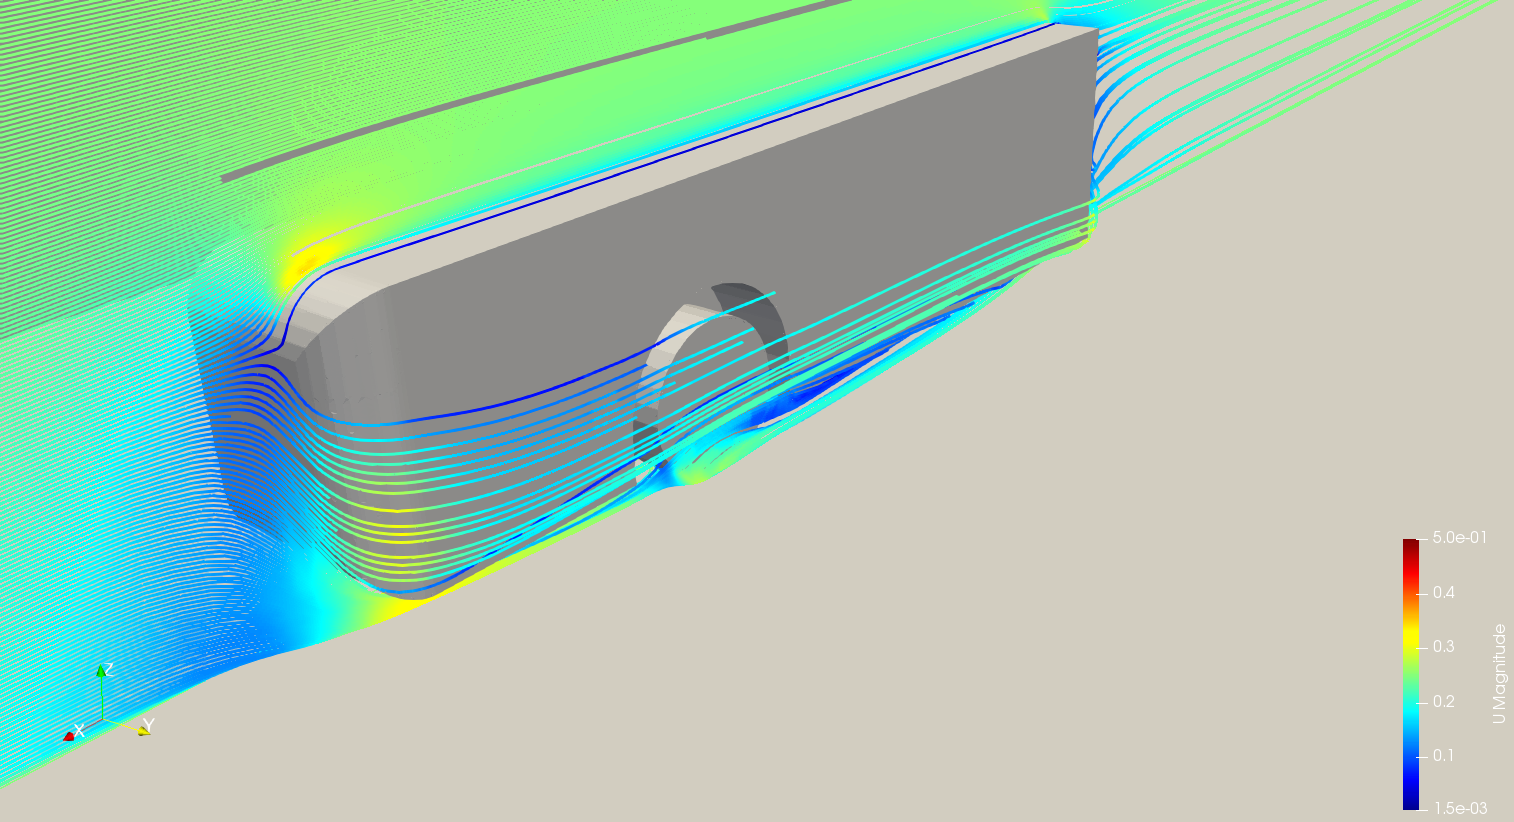
\includegraphics[width=70mm]{screenshots/fullmodel_stream.png}
        \caption{stream of full model}
    \end{center}
\end{figure}
\subsection{今後の課題}
今回は「解析を実行した」のみにとどまってしまったため,
今後は解析結果や解析の条件の分析に努めたい.
分析の内容として,以下のような項目が挙げられる.
\begin{itemize}
    \item 乱流モデルの違いが計算結果に与える影響
    \item 要素数の違いが計算結果及び計算速度に与える影響
    \item メッシュ設定の違いが計算結果に与える影響(境界層・細分化部分の指定 等)
    \item 境界条件の違いによる流れ場への影響
\end{itemize}
\par
分析の方法としては,人間の目では認知できない微妙な違いを判別する必要が
出てくる場合も考えられるため,画像処理を用いて行おうと考えている.
\par
また,数値解析における最大の難点として,計算に長時間必要であることが挙げられるが,
近年では,GPUを用いた並列計算の手法も開発されつつあり,
<<<<<<< HEAD
利用することができれば大幅な計算時間の短縮が期待できる.
長期的な展望としていつか挑戦してみたい.
\subsection{解析における疑問点}
\section{\large opencvを用いた動体検知}
=======
利用することができれば大幅な計算時間の短縮が期待できると考えられる.\\
\subsection{解析における注意点及び疑問点}
\noindent【注意点】
\begin{itemize}
    \item FreeCADでモデルを作成する場合は,stlファイルでエクスポートした際に,
          寸法が1000倍になるためスケール倍率を変更する必要がある.
    \item 境界条件等の設定を含む"0"のフォルダは,解析中に書き換えられる可能性があるため,
          "0.orig"等の名前でフォルダのコピーを作成しておくと良い.
\end{itemize}
\noindent【疑問点】
\begin{itemize}
    \item メッシュの境界面への名前の付け方\\
          (一体で作成したモデルをタイヤモデルと\\ \quad ホイールハウスに名前を別々につける 等)
    \item 計算過程の残差のグラフ表示
    \item 解析結果の収束自動判定
    \item 効果的な解析画像の撮り方
    \item 解析結果の分析のセオリー
    \item 非定常解析の方法
    \item movingWallVelocityとrotatingWallVelocity\\の条件の違い
\end{itemize}
\section{今後の予定}
\begin{itemize}
    \item 作用力測定の実験補助
    \item OpenFOAMを用いた解析
\end{itemize}
>>>>>>> 0d79ce06d5bb38ba77d292d05b35ff3cc34c0b55
\end{document}